\documentclass{article}

% if you need to pass options to natbib, use, e.g.:
%     \PassOptionsToPackage{numbers, compress}{natbib}
% before loading neurips_2018

% ready for submission
% \usepackage{neurips_2018}

% to compile a preprint version, e.g., for submission to arXiv, add add the
% [preprint] option:
%     \usepackage[preprint]{neurips_2018}

% to compile a camera-ready version, add the [final] option, e.g.:
%\usepackage[final]{nips_2018}

% to avoid loading the natbib package, add option nonatbib:
%     \usepackage[nonatbib]{neurips_2018}

\usepackage[utf8]{inputenc} % allow utf-8 input
\usepackage[T1]{fontenc}    % use 8-bit T1 fonts
\usepackage{hyperref}       % hyperlinks
\usepackage{url}            % simple URL typesetting
\usepackage{booktabs}       % professional-quality tables
\usepackage{amsfonts}       % blackboard math symbols
\usepackage{nicefrac}       % compact symbols for 1/2, etc.
\usepackage{microtype}      % microtypography
\newcommand\tab[1][1cm]{\hspace*{#1}}
\usepackage{bm}
\usepackage{amsmath}
\usepackage{amssymb}
\usepackage{amsthm}
\usepackage{graphicx}
\usepackage{bbold}
\usepackage{lmodern}
\title{Speaker ID with the TIMIT Dataset}

\author{
  Team members: Xinlin Chen, Jessica Centers, and Michael Martinez 
}

\begin{document}

\maketitle
\section*{}
\begin{abstract}
The TIMIT database contains clean audio from 630 speakers reading ten phonetically rich sentences. 
The goal of this project was to evaluate various neural network (NN) architectures and feature spaces for the purpose of speech-independent speaker identification on this dataset. 
We evaluates three feature spaces, which we describe as our three methods. 
The first method was to extract common speech features such as mel-frequency cepstral coefficients (MFCCs), delta, and deltaDelta coefficients gathered from the audio clips and use those as the input to a neural network. 
The second method required generating the audio spectrograms and using those 2-D representations of the speech as input to a neural network. 
The third method takes an end-to-end deep neural network approach and uses the raw audio data as the input. 
The use of an autoencoder was also explored. 
For simplicity, the number of speakers considered was reduced to 20, which were randomly selected. 
Based on our experiments, the best feature space to use in a speaker ID neural network was [insert result] as it provided [insert result] accuracy for the 20 speaker subset. 
\end{abstract}
\newpage

\section{Introduction}
\subsection{Motivation and Importance of the Problem}
Speaker identification (ID) is critical to authentication and surveillance applications. 
Example applications include detecting an enemy upon interception of their communication signal, allowing your Amazon Echo or Alexa to identify users that are allowed to command it, or bank account holder verification for transactions being initiated over a phone call.
In many scenarios, including over-the-phone listening, speaker identification is limited to only the acoustic-based identification approach. Scenarios in which other biometric measurements would be used to perform speaker identifcation can easily be argued.
For the sake of this project, it is assumed that the acoustic data of a person speaking is the only biometric measurement available and/or favorable for a speaker ID classifier.
Initial speaker ID classifiers did not use neural networks (NNs), however, the performance of NN based approaches have surpassed traditional approaches according to the technical literature.
For that reason, the goals of this project were to evaluate the performance of different:
\begin{enumerate}
  \item input feature spaces to a speaker ID neural network.
  \item speaker ID neural network architectures for specific input feature.
\end{enumerate}
\subsection{Description of the TIMIT Database}
The TIMIT Acoustic-Phonetic Continuous Speech Corpus was designed specifically to provide speech data for acoustic-phonetic studies and for the development/evaluation of automatic speech recognition systems. 
The speech data is sampled at a rate of 16kHz and the speech sentence lengths of both the training and testing subsets can be seen in the histograms below. 
Also shown is the distribution of speakers by dialect and gender.
\begin{figure}[h!]
  \centering
  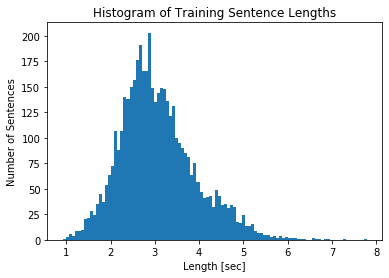
\includegraphics[scale=0.32]{train_hist.png}
  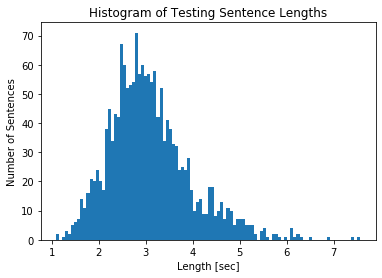
\includegraphics[scale=0.32]{test_hist.png}
  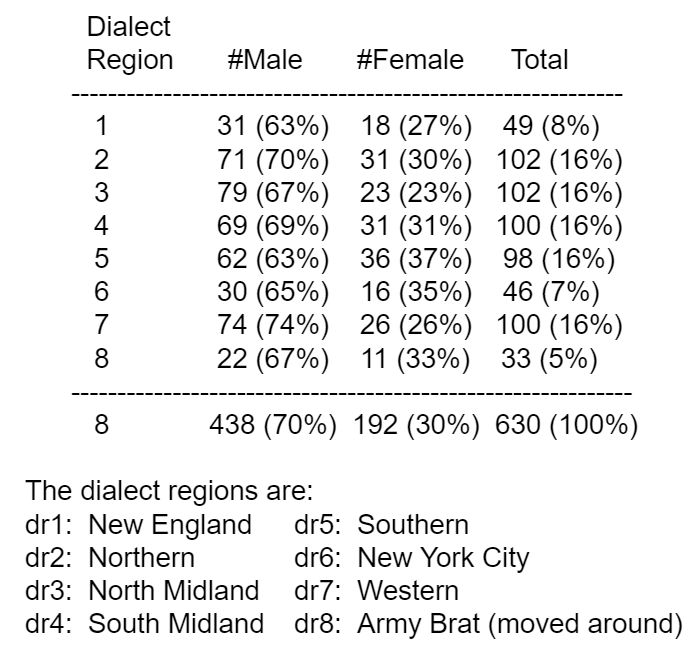
\includegraphics[scale=0.35]{speaker_dist.png}
  \caption{Statistical graphics of TIMIT database characteristics.}
  \label{fig:timit_graphics}
\end{figure}
The TIMIT database is provided in training and testing subsets, however the speech was combined and re-divided into these subsets for this project because the original divide has no speaker in both the training and testing subsets.
Since each speaker contributes 10 sentences to the database, sentences per speaker were separated into training and testing sentences such that there were 7 sentences in training and 3 in testing. \cite{TIMIT}
For use of the TIMIT database, the TIMIT utility library was used. The code provided through this library allowed us to easily load, parse, and use the TIMIT database. \cite{TIMIT_Utils}
\subsection{Overview of Methods}
Three features spaces were explored for the speaker ID classifier that is this project.
\begin{enumerate}
  \item Common speech features described in the technical literature were extracted from each speech data segment and used as the input to the neural network. Features such as the Mel-Frequency Cepstral Coefficients and its Deltas are two of the most common acoustic features considered.
  \item Speech was processed into a 2-D representation that is its spectrogram and that 2-D representation for each the speech data segments was used as the input to the neural network. Various frequency-time representations were considered in creating the spectrograms.
  \item The time-series data or simple transforms of the time-series data for each speech data segment was used as the input to the neural network.
\end{enumerate}

\section{Related Works}
The literature used for each method, as described in the section above, are described below.
\subsection{Method 1: Related Works}
Janet's lit review
\subsection{Method 2: Related Works}
Jessica's lit review
\subsection{Method 3: Related Works}
Michael's lit review

\section{Details of the Project}
For all methods that were experimentally evaluated for this project, a few data organization techniques were kept common. 
Additionally, more traditional classifiers were used as baselines to performance expectations.
\subsection{Data Splitting}
Throughout the literature review, we found the number of seconds considered per data segment varied. 
For this reason, the different methods considered a number of segment lengths experimentally. 
For generalization, say data segments were desired to be $L$ seconds long. 
An additional parameter was introduced to indicate how many $L$-second speech segments should be randomly selected from a speaker. 
This parameter $n$ was calculated based on the average number of seconds a speaker collectively had within the training and testing subsets. 
This average length of speech data per speaker was 31 seconds. 
Then, $n$ was selected to be some integer multiple of 31. 
The results of each method will describe what integer multiple was used. 
In general, selecting $n$ is a matter of trying to have enough samples per speaker in order to do classification while also not over-sampling and therefore causing the neural network to over-fit to the specific sentences within the training subset.
\subsection{Scaling for the Number of Speakers}
Because speaker identification is not expected to work well for the full 630 speakers if it can't work well for fewer speakers, we decided to reduce the number of speakers for experimental purposes.
This allowed us to more quickly tune network parameters and explore more network architectures. 
It should be noted that in the literature review as well as our experimental results, we saw that by scaling down the number of speakers within the dataset being used, that the network must also scale down to work properly.
Although many of the papers we reference use very deep networks for speaker identification on this dataset, since we use a fraction of the samples provided due to using less speakers, the number of weights associated with the deep networks becomes too large to be learned.
Quickly, we discovered that this lead to vanishing gradients and our network would begin predicting only a single class resulting in performance around chance. 
We were able to use leaky rectified linear unit (relu) activation functions in the place of or non-leaky relu activation functions and see this behavior improve, but performance only 50 percent than chance, which for 20 speakers was about 7.5 percent accuracy.
From this we discovered that we needed to scale down our network as we scaled down the number of speakers being considered. 
This was done through reducing the number of nodes within layers as well as reducing the number of layers within our network.
\subsection{Baseline Classifier Performance Results}
Michael did some work here.

\section{Contribution of Each Member of the Team}
This section includes each team member's descriptions of their contribution to this project.
\subsection{Xinlin Chen}
Janet's self-described contributions
\subsection{Jessica Centers}
Jessica's self-described contributions
\subsection{Michael Martinez}
Michael's self-described contributions

\section{Experimental Results}
\subsection{Method 1: Results}
Janet's results
\subsection{Method 2: Results}
Jessica's results
- Diagram of best network architecture.
- Description of different spectrograms and the differences in the results they provided.
- Discussion of multi-task learning results.
- Discussion of nesterov momentum
\subsection{Method 3: Results}
Michael's results

\section{Concluding Remarks}



\bibliography{References}
\bibliographystyle{plain}
\newpage
\end{document}